\documentclass[tikz,border=4pt]{standalone}
\usepackage{amsmath,amssymb}
\usetikzlibrary{positioning,arrows.meta,calc,fit}
\begin{document}
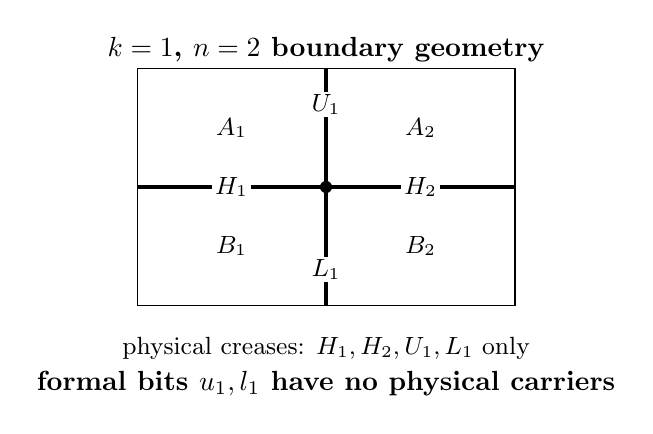
\begin{tikzpicture}[x=1.2cm,y=1.0cm,font=\small]
\node[font=\bfseries] at (2,3.25) {$k=1$, $n=2$ boundary geometry};
\draw (0,1.5) rectangle (2,3);
\draw (2,1.5) rectangle (4,3);
\draw (0,0) rectangle (2,1.5);
\draw (2,0) rectangle (4,1.5);
\node at (1,2.25) {$A_1$}; \node at (3,2.25) {$A_2$};
\node at (1,.75) {$B_1$}; \node at (3,.75) {$B_2$};
% Four and only four physical creases.
\draw[line width=1.4pt] (0,1.5)--(2,1.5); \node[fill=white,inner sep=1pt] at (1,1.5) {$H_1$};
\draw[line width=1.4pt] (2,1.5)--(4,1.5); \node[fill=white,inner sep=1pt] at (3,1.5) {$H_2$};
\draw[line width=1.4pt] (2,1.5)--(2,3); \node[fill=white,inner sep=1pt] at (2,2.55) {$U_1$};
\draw[line width=1.4pt] (2,0)--(2,1.5); \node[fill=white,inner sep=1pt] at (2,.45) {$L_1$};
\fill (2,1.5) circle (2.2pt);
\node[align=center] at (2,-.55) {physical creases: $H_1,H_2,U_1,L_1$ only};
\node[align=center,font=\bfseries] at (2,-1.0) {formal bits $u_1,l_1$ have no physical carriers};
\end{tikzpicture}
\end{document}
